\subsection{Comparison: GRASP vs BRKGA}

In this section we are going to compare the performance of both metaheuristic algorithms applied to the assignment problem.\\
In order to do that, we are first going to choose the best parameters for each algorithm using the large set of problem instances described previously to execute several times each algorithm. The procedure consists of execution the same subset of samples drawn from the large set of problem instances for different proposed values of each parameter tested. The executions can be performed in different computers since the time is not important, only the objective function. The only caveat, is that all parameter values have to solve the same set of instances, since we use the average of objective functions. Otherwise the results would not be coherent from one parameter value to another. We record the objetive function for each execution and compute its average for each parameter value. Then we plot its evolution. We choose the parameter that produces the minimum objective function average.\\
Finally, we will use the best parameter values for each algorithm, to  compare the performance of both algorithm solving the same problem instance.


\subsubsection{Tuning GRASP parameters}

For the parameters of the GRASP algorithm, we have tested the $\alpha$, the $maxIterations$ of the main loop and the $failedIterations$ for the final and more intensive local search.\\
The results of the tests are shown in figure~\ref{fig_grasp_params} on page~\pageref{fig_grasp_params}.

\begin{figure}[h!]
\begin{subfigure}[b]{.49\linewidth}
\centering
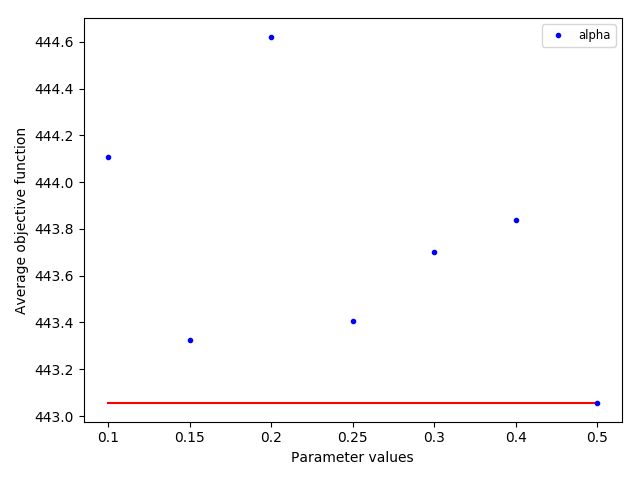
\includegraphics[width=0.8\linewidth]{./img/best-alpha.png}
\caption{ Parameter $\alpha$}\label{fig1a}
\end{subfigure}\hfill
\begin{subfigure}[b]{.49\linewidth}
\centering
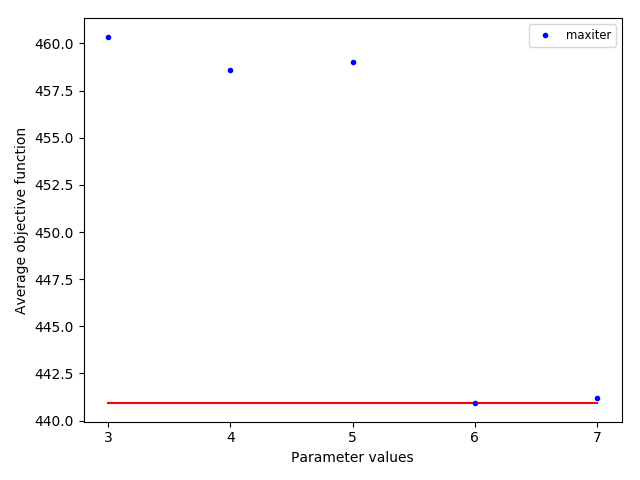
\includegraphics[width=0.8\linewidth]{./img/best-maxiter.png}
\caption{Parameter $maxIterations$ }\label{fig1b}
\end{subfigure}\vfill
\begin{subfigure}[b]{.49\linewidth}
\centering
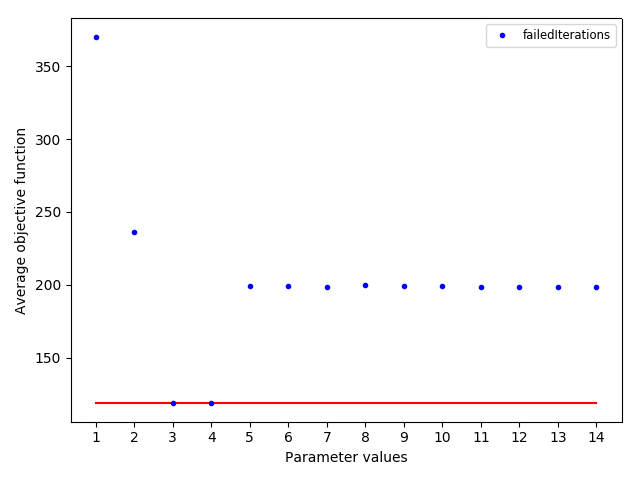
\includegraphics[width=0.8\linewidth]{./img/best-lsiteration.png}
\caption{Parameter $failedIterations$ }\label{fig1c}
\end{subfigure}%
\caption{Average objective function for different \subref{fig1a} $\alpha$, \subref{fig1b} $maxIterations$ and  \subref{fig1c} $failedIterations$ values.  }
\label{fig_grasp_params}
\end{figure}


\pagebreak

\subsubsection{Tuning BRKGA parameters}

For the parameters of the BRKGA algorithm, we have tested the number of generatons ($generations$), the number of individuals in the population ($population$), the inheritance probability ($inheritance$), the proportion of elite individuals in each generation ($eliteprop$) and the proportion of mutant individuals in each generation ($mutantprop$). The results of the tests are shown in figure~\ref{fig_brkga_params} on page~\pageref{fig_brkga_params} .\\

\begin{figure}[H]
\begin{subfigure}[b]{.49\linewidth}
\centering
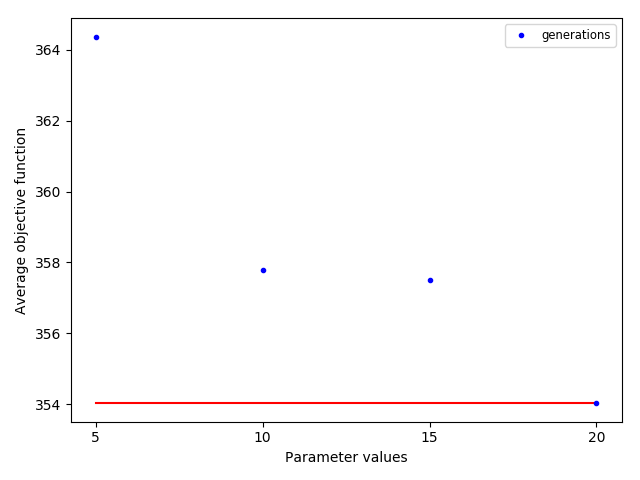
\includegraphics[width=0.8\linewidth]{./img/best-generation.png}
\caption{ Parameter $generations$}\label{fig2a}
\end{subfigure}\hfill
\begin{subfigure}[b]{.49\linewidth}
\centering
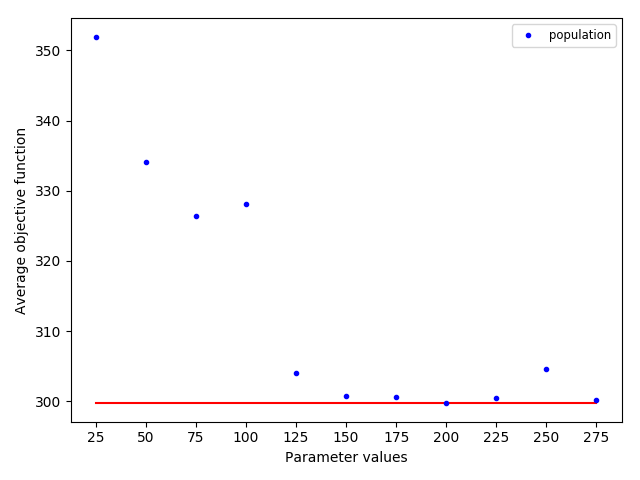
\includegraphics[width=0.8\linewidth]{./img/best-population.png}
\caption{Parameter $population$ }\label{fig2b}
\end{subfigure}\vfill
\begin{subfigure}[b]{.49\linewidth}
\centering
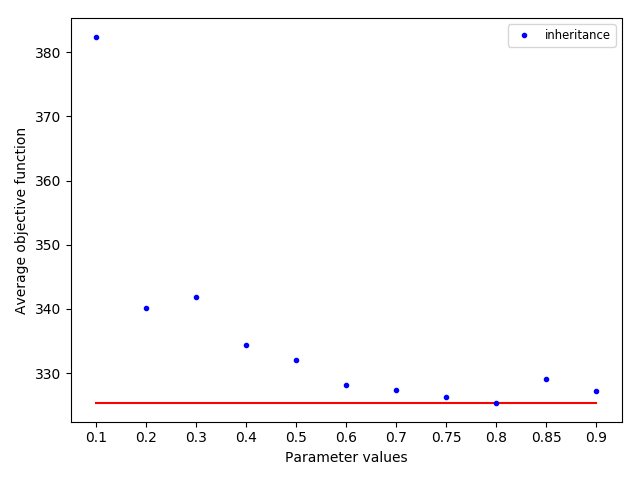
\includegraphics[width=0.8\linewidth]{./img/best-inheritance.png}
\caption{Parameter $inheritance$ }\label{fig2c}
\end{subfigure}%
\begin{subfigure}[b]{.49\linewidth}
\centering
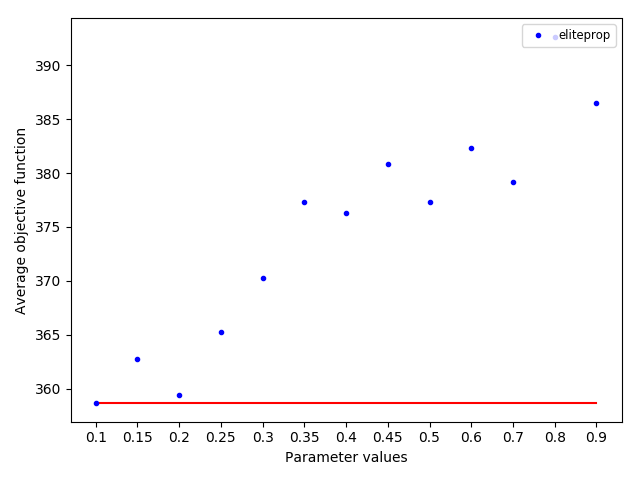
\includegraphics[width=0.8\linewidth]{./img/best-eliteprop.png}
\caption{Parameter $eliteprop$ }\label{fig2d}
\end{subfigure}\vfill
\begin{subfigure}[b]{.49\linewidth}
\centering
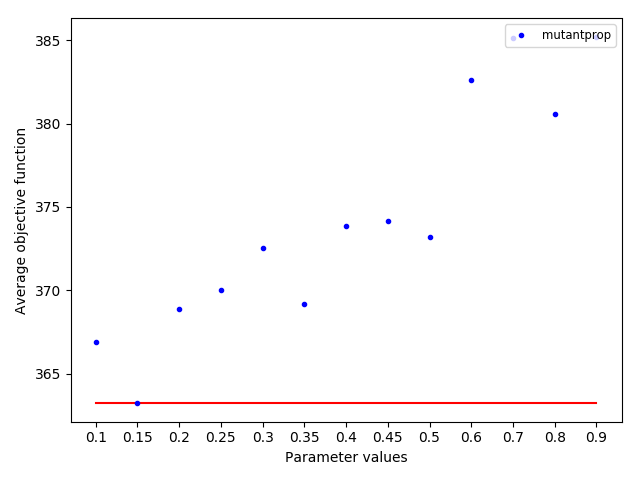
\includegraphics[width=0.8\linewidth]{./img/best-mutantprop.png}
\caption{Parameter $mutantprop$ }\label{fig2e}
\end{subfigure}%
\caption{Average objective function for different \subref{fig2a} $generations$, \subref{fig2b} $population$, \subref{fig2c} $inheritance$, \subref{fig2d} $eliteprop$ and \subref{fig2e} $mutantprop$ values.  }
\label{fig_brkga_params}
\end{figure}





\subsubsection{Comparative results of meta-heuristics performance}

Choosing the best performing parameter setup of the two models, we performed a comparison of how objective function evolves in relation to time.

The output of the parameter selection experiments is the following: 


\begin{tabular}{ll}
GRASP &  BRKGA \\
 $\alpha$ = 0.5  &  $generations$ = 20 \\
 $maxIterations$ = 8 &  $population$ = 200 \\
 $failedIterations$ = 4 & $inheritance$ = 0.8 \\
 						&  $eliteprop$ = 0.1 \\
 						& $mutantprop$ = 0.15 \\


\end{tabular}

Finally, we execute the same problem instance from the large set with both GRASP and BRKGA models. The selected problem instance is the following:
\begin{itemize}
	\item i\-ng\-60\-1600\-1000\-72h\-27mxP\-13mxc\-6mxH\-4mnH\-3Cnt\-20180105\_12\-31\-30343\.dat
\end{itemize}



\begin{figure}[h!]
\centering
\begin{subfigure}[b]{.8\linewidth}

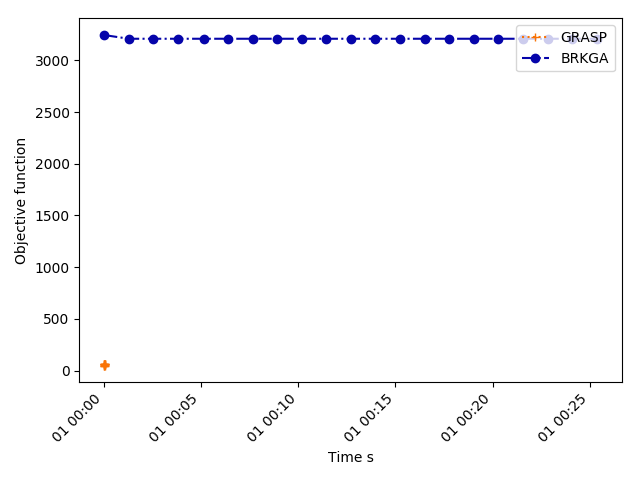
\includegraphics[width=\linewidth]{./img/metah_comparison_objfunc.png}
\caption{ Plot of the evolution of objective function values of the GRASP and BRKGA models }\label{fig1a}
\end{subfigure}%
% \begin{subfigure}[b]{.49\linewidth}
% \centering
% 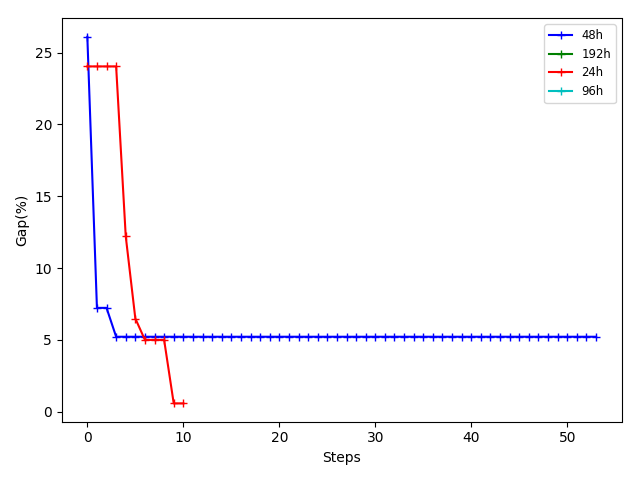
\includegraphics[width=\linewidth]{./img/instances_hours_ilp_evol.png}
% \caption{ Evolution of Gap of the ILP model with different number of hours }\label{fig1b}
% \end{subfigure}\vfill
% \caption{Evolution of Gap of the ILP model with different values of number of nurses (\subref{fig1a}) and number of hours (\subref{fig1b}). }
\label{meta_comparison}
\end{figure}



As we can observe in the chart, the BRKGA model finds the optimal in the fourth generation but it is setup to do twenty generations. This is caused by the fact that we have tested the parameters in isolation. We have not taken into account their interactions and strange results can appear like this early optimal finding of the BRKGA.
We can also appreciate that the BRKGA model starts by having a fitness diversity of 25\% of the total population. Then it gets more than 50\% diversification in the middle generations and then it decreases slowly until the last generation where the diversity is minimum.
An improvement that could be implemented is, as is done in the intensive localsearch, introduce a limited number of non improving iterations upon which the algorithm stops.




Based on the results, we draw conclusions about, why one is better than the other, why one stops sooner than the other. We think in terms of diversification and intensification and solution space exploration.\\

\pagebreak